\documentclass{beamer}
% This is the file main.tex
%\usetheme{default}
\usetheme{Frankfurt}
\usecolortheme{seahorse}
\usecolortheme{rose}
\usefonttheme[onlylarge]{structuresmallcapsserif}
\usefonttheme[onlysmall]{structurebold}
\setbeamerfont{title}{shape=\itshape,family=\rmfamily}
\setbeamercolor{title}{fg=red!80!black}
\setbeamercolor{title}{fg=red!80!black,bg=red!20!white}

% Utilizamos el paquete para usar español
\usepackage[spanish]{babel}
% Utilizamos un paquete para gestionar los acentos
% y las eñes
\usepackage[utf8]{inputenc}
% Utilizamos el paquete para gestionar imagenes jpg
\usepackage{graphicx}
%\usepackage{fancybox}

%\usepackage{fancyvrb}

\usepackage{multimedia}
\usepackage[3D]{movie15}
%\usepackage{multimedia}
\usepackage{hyperref}


\title[Proyecto LAGO]{Nueva electr\'onica para LAGO}
\subtitle{UIS - Colombia}
\author[\texttt{lharnaldi@cab.cnea.gov.ar}]{Ing. Horacio Arnaldi \\ \texttt{lharnaldi@cab.cnea.gov.ar}}
\institute[LabDPR]{Laboratorio Detecci\'on de Part\'iculas y Radiaci\'on \\
   Centro At\'omico Bariloche \\
   Comisi\'on Nacional de Energ\'ia At\'omica}
%\author{Ing Horacio Arnaldi}
\date{\today}

\begin{document}
\begin{frame}
  \hspace*{0.2cm}
  
\includegraphics[height=0.2\textheight]{../media/cnea_logo.jpg} \hspace*{1cm}
  
\includegraphics[height=0.2\textheight]{../media/balseiro_logo.jpg} \hspace*{1cm}
  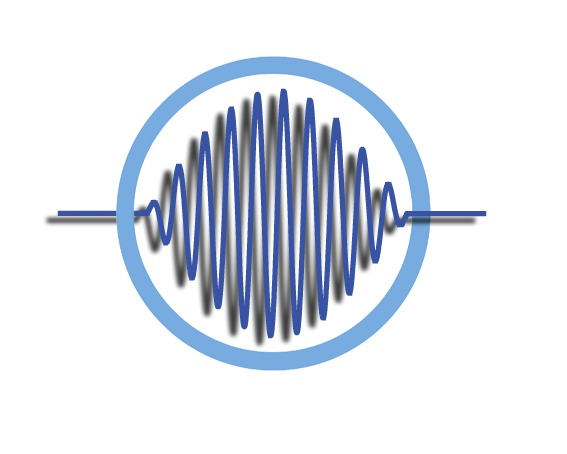
\includegraphics[height=0.2\textheight]{../media/LabDPR_logo.jpg} \hspace*{1cm}
  
\includegraphics[height=0.18\textheight,width=0.15\textwidth]{../media/lagologo.jpg}

	\titlepage

\end{frame}

\section*{Outline}
\begin{frame}
	\tableofcontents[pausesections]
\end{frame}

\section{¿Qué es LAGO?}
\begin{frame}
	\frametitle{¿Qué es LAGO?}
	\framesubtitle{\textit{Large Aperture Gamma Ray Burst Observatory}}

\end{frame} 

\begin{frame}
	\frametitle{¿Qué es LAGO?}
	\framesubtitle{\textit{Large Aperture Gamma Ray Burst Observatory}}

\begin{columns}
	\begin{column}{0.40\textwidth}
		\begin{block}{Varios sitios (\textgreater4000msnm)}
    	\begin{itemize}[<+->]
      	\item  México (Cerro La Negra)
      	\item  Bolivia (Chacaltaya)
      	\item  Venezuela (Mérida)
				\item  Argentina (Auger)
				\item	 Ecuador (Chimborazo)
    	\end{itemize}
		\end{block}
	\end{column} 
 	\begin{column}{0.55\textwidth}
  	\includegraphics[width=\textwidth]{../media/sitios_lago.jpg}
 \end{column}
\end{columns}
\end{frame} 

\begin{frame}
	\frametitle{Detectores Cherenkov}
	\framesubtitle{PMT}
\begin{columns}
	\begin{column}{0.50\textwidth}
  	\fbox{\includegraphics[width=\textwidth]{../media/pmt_otro_inet.jpg}}
	\end{column} 
 	\begin{column}{0.50\textwidth}
  	\fbox{\includegraphics[width=0.7\textwidth]{../media/divisor_pmt.jpg}}
 \end{column}
\end{columns}
\end{frame} 

\begin{frame}
	\frametitle{Detectores Cherenkov}
	\framesubtitle{PMT}
\begin{columns}
	\begin{column}{0.50\textwidth}
  	\fbox{\includegraphics[width=0.8\textwidth]{../media/nahuelito.jpg}}
	\end{column} 
 	\begin{column}{0.50\textwidth}
  	\fbox{\includegraphics[width=\textwidth]{../media/fototubo_pmt.jpg}}
 \end{column}
\end{columns}
\end{frame} 

\section[Lo que teníamos]{¿Qué teníamos hasta ahora?}
\begin{frame}
	\frametitle{¿Qué teníamos hasta ahora?}

\begin{columns}
	\begin{column}{0.40\textwidth}
		\begin{block}{Electrónica dedicada para Auger}
    	\begin{itemize}[<+->]
      	\item Poco flexible 
      	\item Información limitada
      	\item Número limitado de UB 
				\item Comunicación de datos por puerto serie
				\item	Tiempos de adquisición largos
				\item	Poco volumen de almacenamiento
				\item Sin control línea de base	
    	\end{itemize}
		\end{block}
	\end{column} 
 	\begin{column}{0.55\textwidth}
  	\fbox{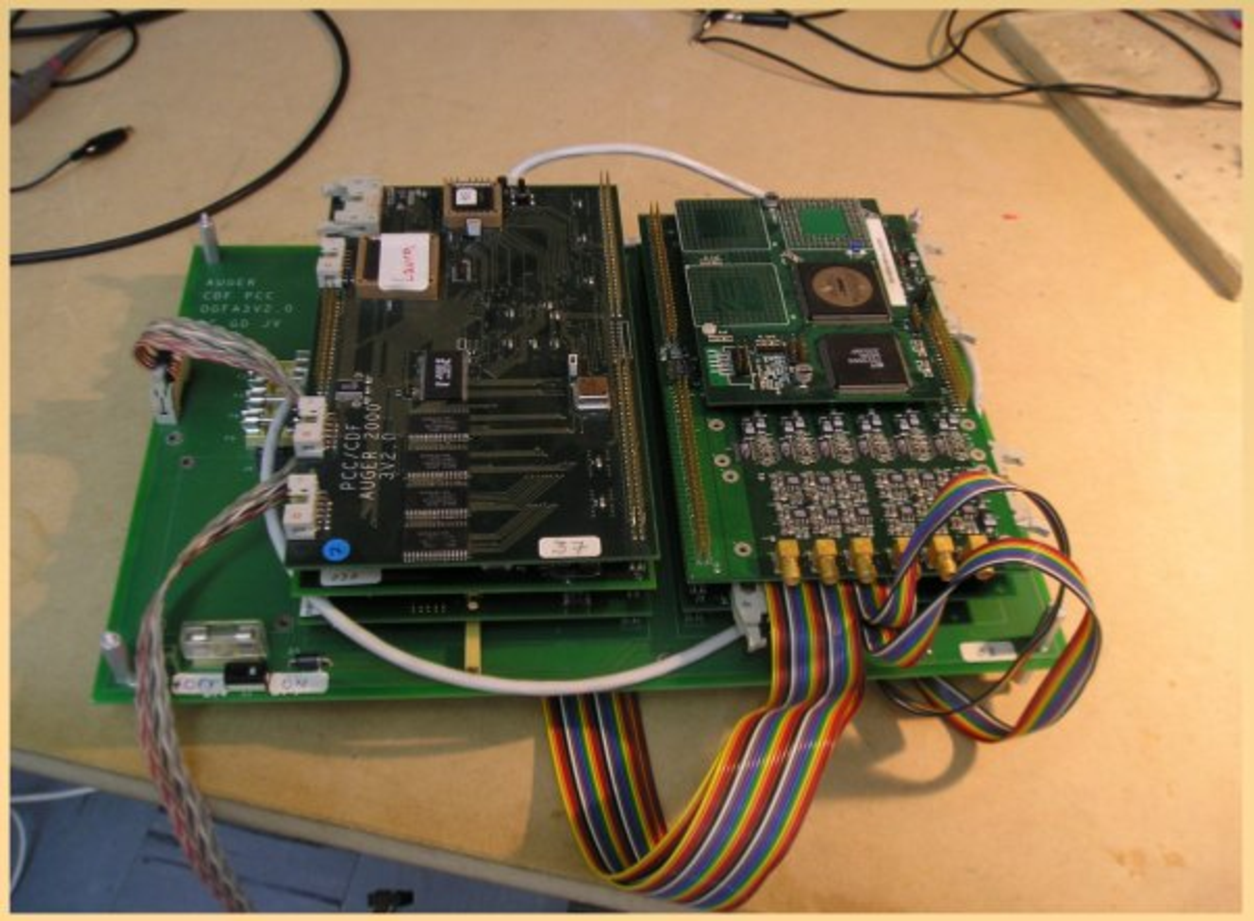
\includegraphics[width=\textwidth]{../media/electronica_auger.jpg}}
 \end{column}
\end{columns}
\end{frame} 

\section{¿Qué queremos?}
\begin{frame}
	\frametitle{¿Qué queremos?}
		\begin{block}{}
    	\begin{itemize}
      	\item Obtener la mayor cantidad de información
							posible con el menor costo (pulsos, tiempo
							entre pulsos, amplitudes para frecuencias
							altas de pulsos, etc) 
      	\item Sincronización de los diferentes sitios
      	\item Sistema adaptable a otros experimentos
    	\end{itemize}
		\end{block}
\end{frame} 

\section[Propuesta]{¿Qué proponemos?}

\begin{frame}
	\frametitle{¿Qué proponemos?}

\begin{columns}
 	\begin{column}{0.55\textwidth}
  	\fbox{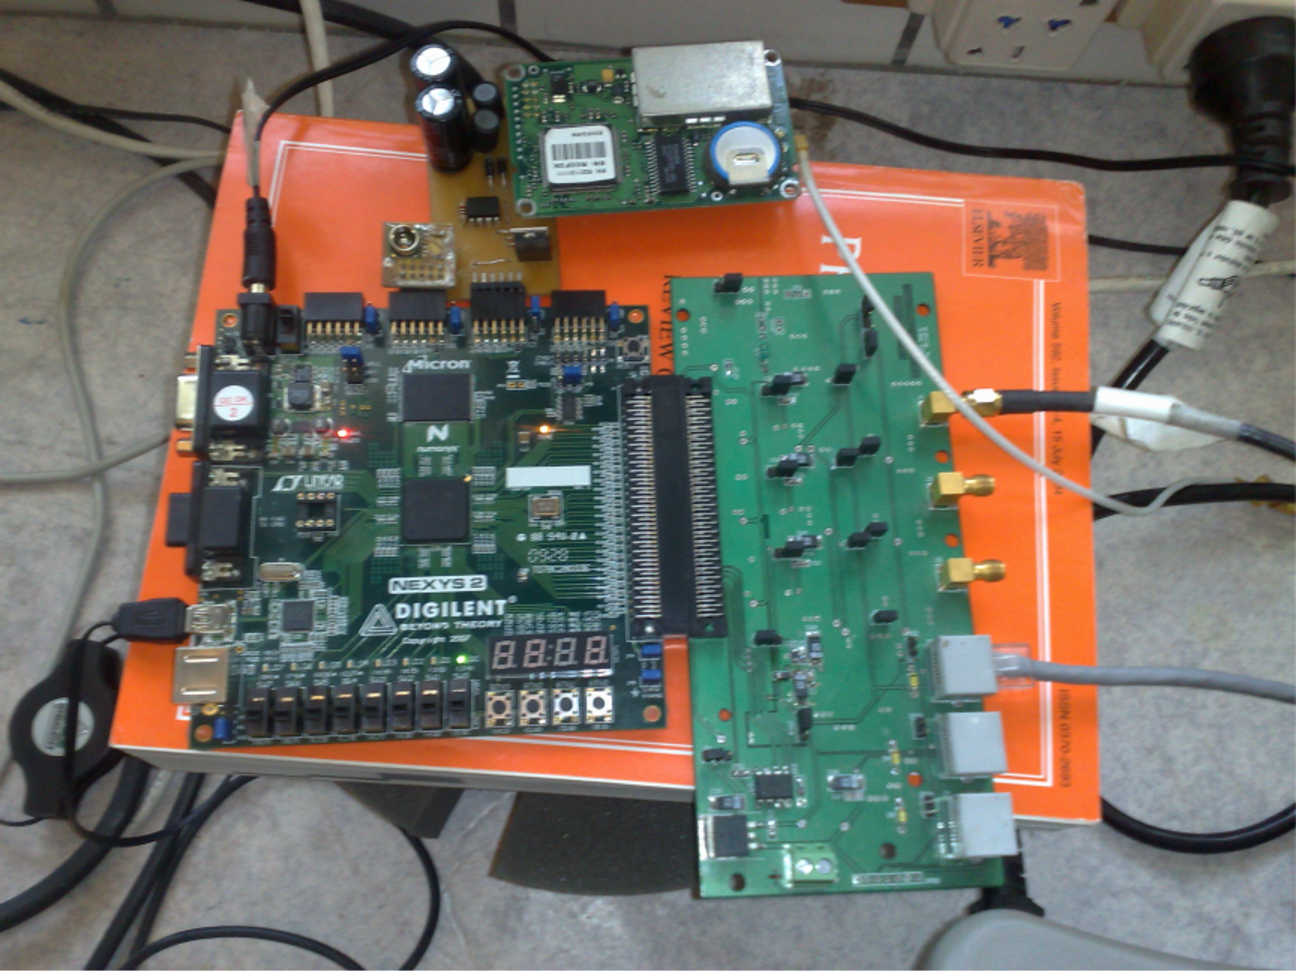
\includegraphics[width=\textwidth]{../media/hardware_nahuelito.jpg}}
 \end{column}
	\begin{column}{0.40\textwidth}
		\begin{block}{}
    	\begin{itemize}[<+->]
      	\item Placa de digitalización de tres canales
      	\item GPS para sincronizar los datos de los 
							distintos sitios
      	\item Barómetro 
				\item Placa Nexys2 (FPGA Spartan 3E)
    	\end{itemize}
		\end{block}
	\end{column} 
\end{columns}
\end{frame} 

\section{¿Cómo se logró?}

\begin{frame}
	\frametitle{Placa de digitalización}
\begin{columns}
	\begin{column}{0.40\textwidth}
		\begin{block}{Características}
    	\begin{itemize}[<+->]
      	\item 3 canales
      	\item ADC de 10 bits
      	\item 40 MSPS 
				\item Pulse shaper
				\item Control activo de la línea de base
				\item Control de alta tensión para base de PMT
    	\end{itemize}
		\end{block}
	\end{column} 
 	\begin{column}{0.55\textwidth}
  	\only<1-3>{\fbox{\includegraphics[width=0.7\textwidth]{../media/placa_lago.jpg}}}
  	\only<4-6>{\fbox{\includegraphics[width=\textwidth]{../media/newel_frente.jpg}}}
 \end{column}
\end{columns}
\end{frame} 

\begin{frame}
	\frametitle{Diagrama en bloques}
	\begin{block}{}
  	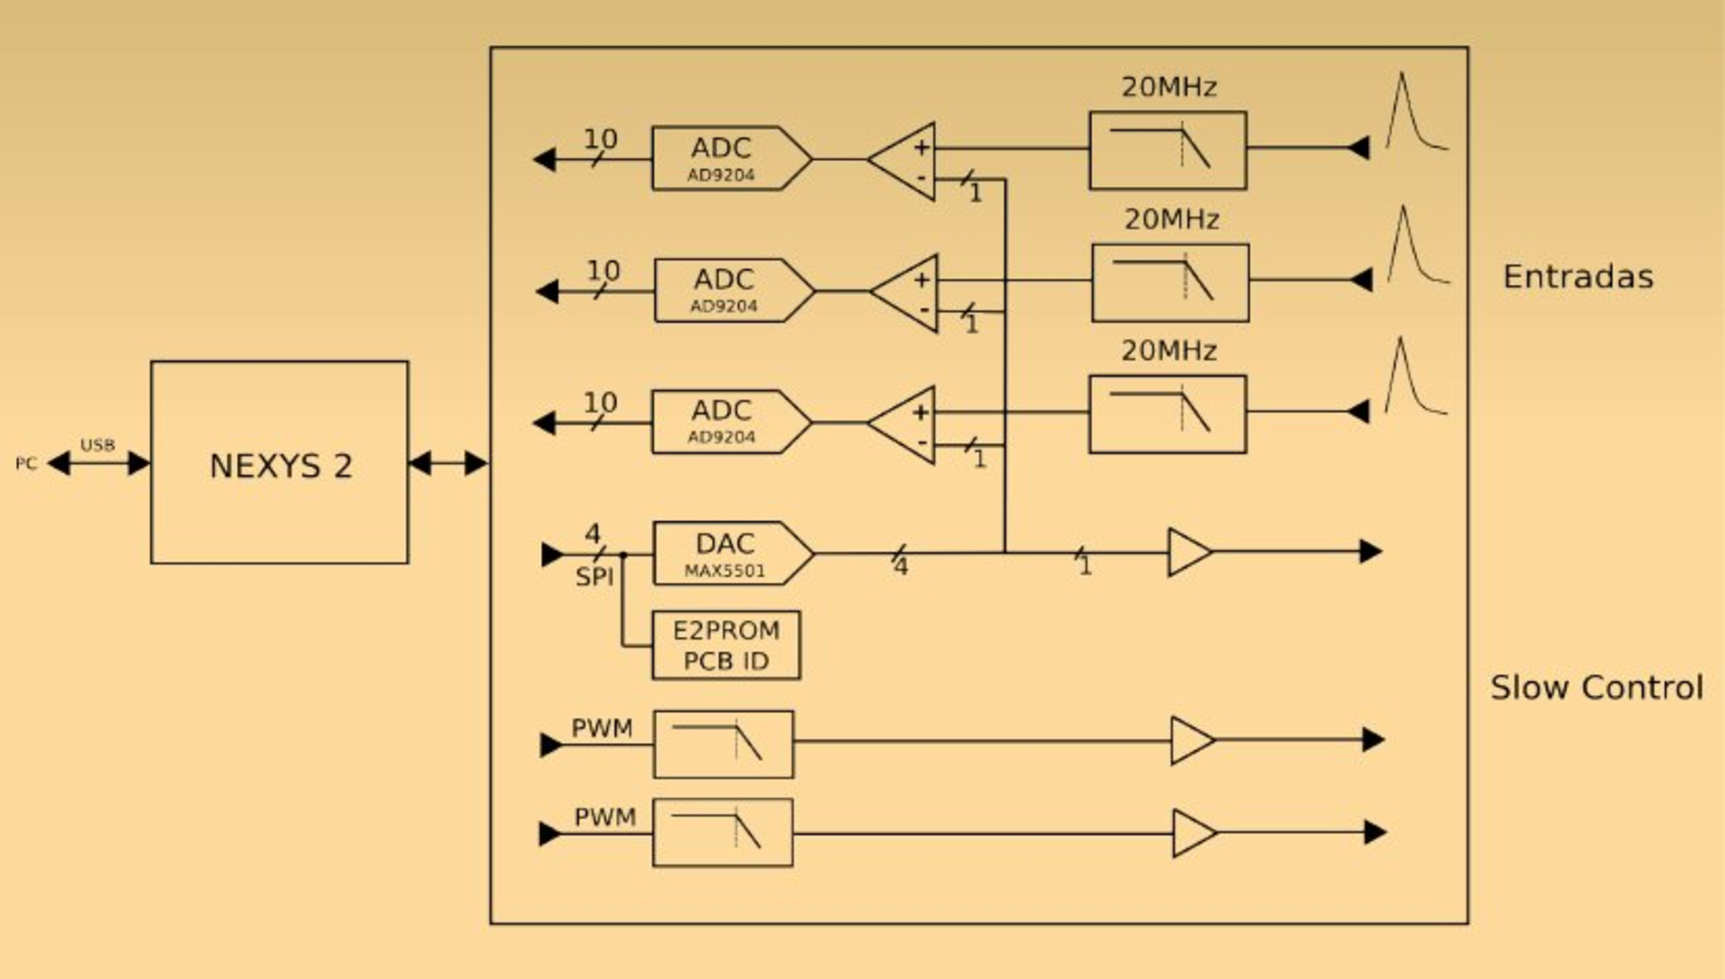
\includegraphics[width=\textwidth]{../media/diagrama_en_bloques_lago.jpg}
	\end{block}
\end{frame} 

\begin{frame}
	\frametitle{Front-end}
	\begin{block}{}
  	\includegraphics[width=\textwidth]{../media/front_end_lago.jpg}
	\end{block}
\end{frame} 

\begin{frame}
	\frametitle{Bloques en la FPGA}
%	\begin{block}{}
	\begin{center}
  	\fbox{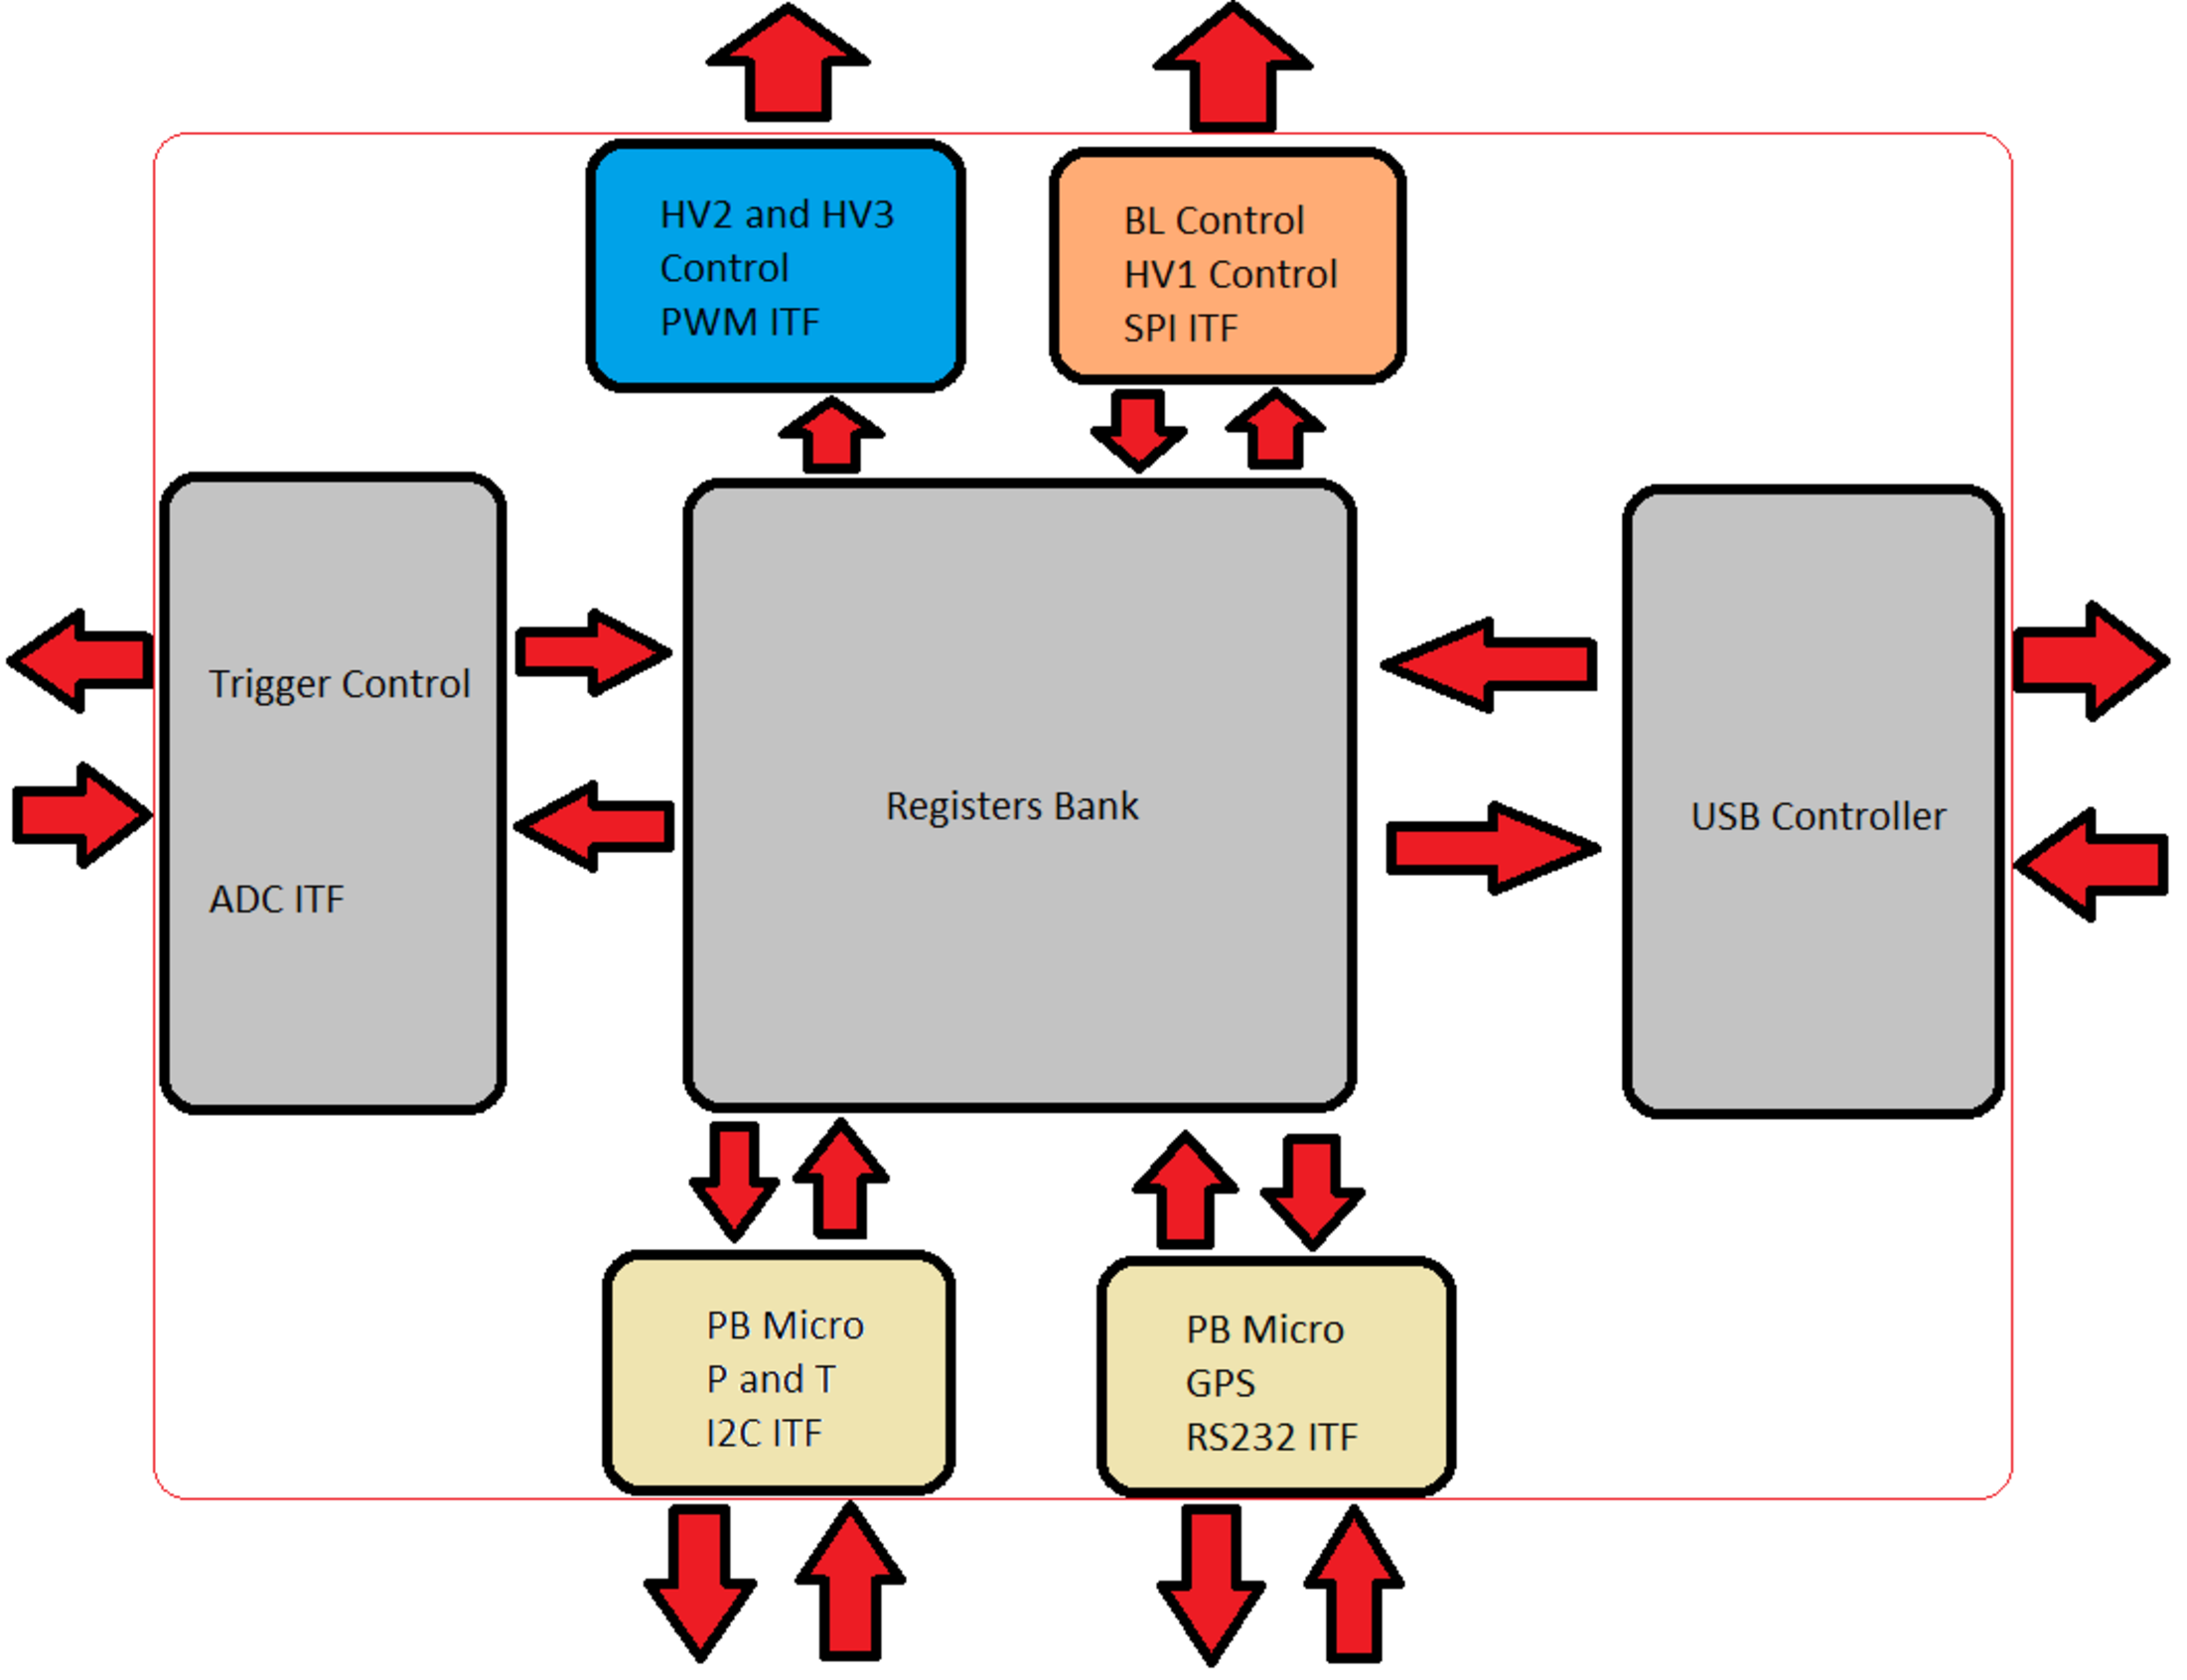
\includegraphics[width=0.8\textwidth]{../media/bloques_fpga_lago}}
	\end{center}
%	\end{block}
\end{frame} 

\begin{frame}
	\frametitle{Estándares implementados en la FPGA}
		\begin{block}{}
    	\begin{itemize}
      	\item Interfaz SPI para el control de la línea 
							de base del sistema a través de un DAC 
      	\item Interfaz I2C para la obtención de los 
							datos del sensor de presión y temperatura
      	\item Interfaz RS232 para la comunicación 
							bidireccional con el receptor GPS
      	\item Interfaz USB bidireccional para la 
							comunicación de datos y el envío de 
							órdenes desde la PC
    	\end{itemize}
		\end{block}
\end{frame} 

\begin{frame}
	\frametitle{Facilidades del código desarrollado}
		\begin{block}{Datos}
    	\begin{itemize}
      	\item GPS
    		\begin{itemize}
 					\item Tiempo en formato UTC o GPS
    		\end{itemize}
      	\item Presión y temperatura
      	\item 3 canales
      	\item Contador de triggers
      	\item Se puede determinar el canal que tuvo un 
							evento de trigger
      	\item Monitoreo constante del reloj del sistema
    	\end{itemize}
		\end{block}
\end{frame} 

\begin{frame}
	\frametitle{Interfaz USB}
		\begin{block}{Características}
    	\begin{itemize}
      	\item Bus de datos bidireccional de 8 bits
 				\item 6 líneas de control (handshaking)
      	\item Transferencia sincrónica de datos
      	\item Velocidad de transferencia de datos en 
							torno a los 25 MB/s
      	\item Utilización de librerías open source LGPL
      	\item Implementado sobre un firmware propio, 
							pero sin borrar el firmware que trae la 
							Nexys2
    	\end{itemize}
		\end{block}
\end{frame} 

\begin{frame}
	\frametitle{Soluciones: El software}
		\begin{block}{Lago.cpp}
    	\begin{itemize}
      	\item Un sólo software para manejar todas las 
							funciones implementadas en la FPGA
 				\item Capacidad de consultar y configurar 
							registros de forma independiente
      	\item Control separado de cada canal
      	\item Adquisición de datos por puerto USB 
      	\item Rate de pulsos de 10 kHz para el modo
							trigger normal y $\approx$ 100 kHz para el modo
							subtrigger
    	\end{itemize}
		\end{block}
\end{frame} 

\begin{frame}
\begin{block}{Pruebas: un ejemplo de análisis online}
\includemovie[poster,label=lago,text=lago.mpg,url,
repeat]
{.5\linewidth}{.375\linewidth}{lago.mpg}
\end{block}
\end{frame}

\begin{frame}
	\frametitle{Los datos}
  \begin{itemize}
    \item Presión y temperatura
  \end{itemize}
  	\fbox{\includegraphics[width=\textwidth]{../media/pyt.jpg}}
\end{frame} 

\begin{frame}
	\frametitle{Pruebas}
  \begin{itemize}
    \item Algunas pruebas en el laboratorio
  \end{itemize}
  \begin{center}
  	\fbox{\includegraphics[width=0.8\textwidth]{../media/hard_y_pulso.jpg}}
  \end{center}
\end{frame} 

\begin{frame}
	\frametitle{\ldots más pruebas \ldots}
		\begin{block}{}
    	\begin{itemize}
      	\item Toma de datos en el detector Nahuelito y  
							Boyita realizadas con éxito (Sputnik en 
							etapa de testeo)
 				\item Se caracterizaron los detectores con la 
							nueva electrónica como herramienta
      	\item Hasta ahora la adquisición de datos del 
							tanque nuevo de aluminio no son 
							satisfactorias
      	\item Problemas de excesos de luz, posibles
							problemas de geometría, etc 
    	\end{itemize}
		\end{block}
\end{frame} 

\begin{frame}
	\frametitle{Usos didácticos}
		\begin{block}{}
    	\begin{itemize}
				\item En la materia Experimental III, que se 
							dicta en el IB se usa actualmente la 
							nueva electrónica LAGO para caracterizar 
							y realizar las prácticas con el detector 
							Nahuelito
				\item Los alumnos interactúan con el software 
							y hardware desarrollado 
				\item La nueva electrónica desarrollada abre 
							nuevas posibilidades para el análisis de 
							los datos por parte de los alumnos
    	\end{itemize}
		\end{block}
\end{frame} 

\section[Logros]{Logros iniciales}

\begin{frame}
	\frametitle{Logros iniciales}
		\begin{block}{}
    	\begin{itemize}
				\item Implementación eficiente de un sistema 
							de trigger y subtrigger en la FPGA
				\item Comunicación efectiva de datos a través 
							del puerto USB
				\item Software de control para todas las 
							funciones
				\item La comunidad LAGO está empezando a 
							utilizar la nueva electrónica
				\item GPS integrado
				\item Presión y Temperatura
				\item Control automático de línea de base
    	\end{itemize}
		\end{block}
\end{frame} 

\begin{frame}
	\frametitle{Logros iniciales}
		\begin{block}{}
    	\begin{itemize}
			\item Con las nuevas librerías se consiguió
						mejorar el ancho de banda de transmisión 
						de datos
			\item Contínuamente se prueban variantes al 
						formato de los datos
			\item Actualmente se está trabajando con la 
						versión 2.0 del código de adquisición
			\item Va acompañado de la versión 4.0 para el 
						data file
    	\end{itemize}
		\end{block}
\end{frame} 

\begin{frame}
  \begin{center}
    \huge{¡Muchas Gracias!}
  \end{center}
\end{frame}

\end{document}
